\chapter{基于IMU预积分的目标函数}\label{ch:vislam}

如上一章中提到的,单目VSLAM系统存在一定的局限性,非常依赖相机的成像质量,并且无法绝对尺度进行观测\citep{jones2011visual}。而在移动AR、自动驾驶、无人机等应用中,为了与场景交互或是提供路径规划,SLAM算法必须鲁棒地提供带尺度信息的位姿估计和运动估计。而且随时可能出现的光照、纹理质量的变化,以及相机快速运动带来的图像模糊,都时刻在挑战着相机跟踪算法的鲁棒性。

近些年来,IMU被广泛地与VSLAM系统结合。不管是使用滤波方法还是非线性优化方法实现的VISLAM系统,对IMU的建模都大同小异,基本集中在两类:一类是类似于MSCKF\citep{mourikis2007multi}、OKVIS\citep{leutenegger2015keyframe}那样传统的迭代式IMU积分,另一类则是使用IMU预积分\citep{forster2017manifold}的方法,如VINS\citep{li2017monocular}。

\section{IMU基本模型}

IMU是测量物体三轴角速度以及加速度的装置,包含三轴陀螺仪和线加速度计。IMU工作极其稳定,几乎不会有宕机的情况,而且通常能以远高于相机的频率(数百到上千赫兹)得到相对于自身坐标系的角速度$\bm{\omega}$($rad \cdot s^{-1}$)和加速度$\bm{a}$($m \cdot s^{-2}$)。依靠这些数据,可以通过数值积分计算得到系统的朝向$\mathrm{R}\in\mathbb{SO}^3$、速度$\bm{v}\in\mathbb{R}^3$和平移$\bm{p}\in\mathbb{R}^3$信息,因此基于IMU的跟踪结果直接就带有了场景的尺度信息。很自然地,IMU工作并不依赖于视觉信息,可以在相机遭遇恶劣的光照、纹理以及运动模糊的情况下提供较为可靠的跟踪结果。但值得注意的是,消费级别的IMU传感器,其信号通常带有较大的bias\footnote{指IMU输出值和输入值之间的偏移,可能受温度、重力等因素的影响}和噪声,并且系统的速度$\bm{v}$和平移$\bm{p}$分别来自于加速度$\bm{a}$的一次和二次数值积分,bias和噪声也会通过积分以平方级别被放大,带入到跟踪结果中。因此仅使用IMU的跟踪结果是不可靠的,需要定期使用视觉跟踪信息来纠正IMU跟踪的误差。

鉴于其噪声特性,合理地使用IMU辅助视觉跟踪是一项重大挑战。不管是使用滤波的方法还是非线性优化的方法融合视觉信息和IMU信息,都要对IMU的误差进行合理的建模。将IMU的实际物理运动定义为传感器的输入,IMU对实际运动进行测量得到角速度和加速度定义为传感器输出,则输出和输入的差异即为IMU读数的误差,常见的IMU误差模型可以用图~\ref{fig:common_imu_errors}来表示。

\begin{figure}[htb!]
    \centering
    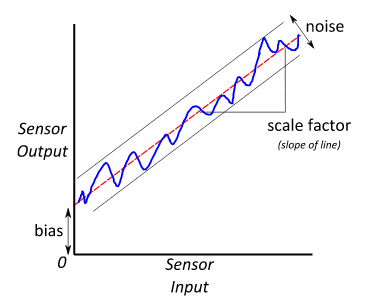
\includegraphics[width=.4\textwidth]{Pictures/common_imu_errors.png}
    \caption{一般的IMU误差模型\citep{imu2014}}
    \label{fig:common_imu_errors}
\end{figure}

可以看到,IMU误差的成分是比较复杂的,可能包含bias、随机游走噪声(random walk)\footnote{指当输入固定时,IMU输出值中包含的随机噪声,它随时间的变化可被认为是一个随机过程}、尺度系数(scale factor)\footnote{指的是输出和输入之间的线性缩放系数}、不正交性(non-orthogonality)\footnote{指由于IMU各轴并不完全正交所带来的误差}等等\citep{imu2014},而不同类型误差对于运动估计的影响也是不同的。在跟踪的过程中,系统的朝向$\mathrm{R}$可以通过角速度$\bm{\omega}$的数值积分得到;加速度$\bm{a}$会被进行一次和二次积分,分别得到速度$\bm{v}$和平移$\bm{p}$。加速度经过了二次数值积分,其误差也会通过两次积分进入平移量$\bm{p}$中,故相比角速度的误差,跟踪算法对于加速度的误差更为敏感。实际经验也表明,由IMU积分得到的朝向信息是较为准确的,而位置信息的误差则是较大的。

一般IMU在出厂时都会经过厂商的校准,故在实际跟踪和状态估计的过程中可以使用一个简化的IMU误差模型。以常用的六轴IMU为例,
大部分的VISLAM系统都使用了相同的IMU误差模型,如MSCKF、VINS-Mono等,即将其误差简化为bias和测量噪声两个部分,并假设加速度计和陀螺仪相互统计独立,且各自的三轴之间都统计独立。使用下标$m$标记每次测量的值,不带下标的表示真实值左上标$^G$来表示参考系为全局坐标系,不带左上标的表示参考系为局部坐标系。在不考虑地球自转的情况下,角速度和加速度的测量分别为:
\begin{equation}
\begin{aligned}
    \tilde{\bm{\omega}}
        &= \bm{\omega} + \bm{b}^g + \bm{n}^g,  \\
    \tilde{\bm a}
        &= \prescript{G}{}{\mathrm{R}^\top}
            (\prescript{G}{}{\bm a} - \prescript{G}{}{\bm{g}}) +
                \bm{b}^a + \bm{n}^a
\end{aligned}
\end{equation}
可以看到,IMU的的读数可以看成是真实值、偏移和加性高斯白噪声(addative Gaussian white noise)之和。而加速度的测量中又包含了重力$\prescript{G}{}{\bm g}$的影响。bias和白噪声具备如下性质:
\begin{itemize}
    \item bias~$\bm{b}^g$和$\bm{b}^a$:随时间的增长符合零均值的高斯随机游走。该噪声从IMU开机以来就一直存在,不断积累,与是否从IMU读取数据无关。可以用如下高斯分布来描述:
        \begin{equation}
        \begin{aligned}
            \bm{b}^g &\sim \mathcal{N}(\bm{b}_0^g, \mathrm{Q}_g), \\
            \bm{b}^a &\sim \mathcal{N}(\bm{b}_0^a, \mathrm{Q}_a)
        \end{aligned}
        \end{equation}
    \item 测量噪声$\bm{n}^g$和$\bm{n}^a$:零均值加性高斯白噪声,表示从IMU读取数据时产生的小抖动,而且这个噪声只在测量时产生,也符合高斯分布:
        \begin{equation}
        \begin{aligned}
            \bm{n}^g & \sim \mathcal{N}(\bm{0}, \mathrm{R}_g), \\
            \bm{n}^a & \sim \mathcal{N}(\bm{0}, \mathrm{R}_a),
        \end{aligned}
        \end{equation}
\end{itemize}
为了方便后续的计算,IMU测量误差的协方差也可以记为:
\begin{equation}
\Sigma =
    \begin{bmatrix}
        \mathrm{Q}_g &            0 &            0 &         0 \\
                   0 & \mathrm{R}_g &            0 &         0 \\
                   0 &            0 & \mathrm{Q}_a &         0 \\
                   0 &            0 &            0 & \mathrm{R}_a
    \end{bmatrix}
\end{equation}

\subsection{离散时间噪声和连续时间噪声}

上面提到的噪声模型都是在连续时间系统下面考虑的,连续时间系统的高斯协方差(或标准差)也就称为传感器的噪声强度。实际应用中,不可能每时每刻都在读取IMU数据,而应该考虑离散时间系统的情况。\citep{smith1978exact}给出了离散时间噪声和连续时间噪声的关系。可知,离散时间系统下IMU噪声的协方差与连续时间系统存在如下关系:
\begin{equation}
\begin{aligned}
    \mathrm{Q}_{gd} &= \mathrm{Q}_g \Delta t   \\
    \mathrm{Q}_{ad} &= \mathrm{Q}_a \Delta t   \\
    \mathrm{R}_{gd} &= \mathrm{R}_g / \Delta t \\
    \mathrm{R}_{ad} &= \mathrm{R}_a / \Delta t
\end{aligned}
\end{equation}
其中$\Delta t$为采样时间间隔,并且陀螺仪、加速度计三轴的噪声统计独立。

\subsection{IMU状态传播}

所谓的IMU状态传播(IMU propagation)指的就是根据通过将当前时刻IMU的读数在时间上进行积分,来得到下一时刻的IMU状态。这个IMU状态包括IMU的位姿、运动以及噪声等,通过积分操作,IMU读数的信息就被传播到了下一时刻。

首先考虑理想情况,也就是IMU的读数不存在白噪声,偏移量也不存在随机游走的情况,此时IMU的读数符合:
\begin{equation}
\begin{aligned}
    \bm{\omega}  &= \tilde{\bm{\omega}} - \bm{b}^g, \\
    \bm{a} &= \tilde{\bm a} - \bm{b}^a + \bm{g}.
\end{aligned}
\end{equation}

记全局坐标系下IMU的状态为(为保持简洁,省略了转置符号${}^\top$):

\begin{equation}
  \bm{X}_{\textrm{IMU}} \doteq
  \left[
      \prescript{G}{}{\mathrm R},
      \prescript{G}{}{\bm p},
      \prescript{G}{}{\bm v},
      \bm{b}^g, \bm{b}^a
  \right].
\end{equation}

具体来说,积分过程包括积分这个IMU状态向量的五个分量。那么,要对IMU状态进行积分,首先需要写出IMU状态关于时间的导数:
\begin{equation}
\begin{aligned}
    \prescript{G}{}{\dot{\mathrm R}}
        &= \prescript{G}{}{\mathrm R} \lfloor(\tilde{\bm{\omega}} - \bm{b}^g)\times\rfloor, \\
    \prescript{G}{}{\dot{\bm p}}
        &= \prescript{G}{}{\bm v}, \\
    \prescript{G}{}{\dot{\bm v}}
        &= \prescript{G}{}{\mathrm R} (\tilde{\bm a} - \bm{b}^a + \bm{g}), \\
    \dot{\bm b}^g &= \bm{0}, \\
    \dot{\bm b}^a &= \bm{0}
\end{aligned}
\end{equation}

显然,由于偏移$\bm{b}^g$和$\bm{b}^a$随时间的增长符合零均值的高斯随机游走,故它们关于时间的导数为零。积分的步骤如下:

\begin{enumerate}
    \item 将角速度在时间上积分,得到当前IMU的朝向;
    \item 将加速度在时间上积分,得到当前IMU的速度;
    \item 将速度再在时间上积分,得到当前IMU的位置;
    \item 角速度偏移和加速度偏移由于增长符合零均值随机游走,所以直接取旧的状态中的值。
\end{enumerate}

可以使用任意一种数值积分算法来实现,比如欧拉法(Euler method)、龙格库塔法(Runge-Kutta methods)等。此外,不仅要对状态向量进行数值积分,同时还要更新协方差矩阵。
  % section : IMU基本模型

\section{基于IMU预积分技术的VISLAM}

接下来重点介绍IMU预积分技术\citep{forster2017manifold}。与普通基于IMU积分的VISLAM系统不同,IMU预积分使用了更精确的相对运动模型。将IMU观测模型包含三个部分:相对旋转、相对速度、相对平移,可以认为它们是仅关于偏移量的函数。使用以下算法进行IMU预积分,假设需要对$t_i$和$t_j$之间IMU读数进行积分(假设相邻两帧IMU之间时间间隔相同,即$\Delta t_{i,i+1} = \Delta t_{i+1,i+2} = \cdots = \Delta t_{j-1,j} = \Delta t$):

\begin{equation}
\begin{aligned}
\mathrm{R}_j &= \mathrm{R}_i \prod_{k=i}^{j-1}
                \exp\left(
                    (\tilde{\bm\omega}_k - \bm{b}_k^g - \bm{n}_k^g) \Delta t
                \right) \\
\bm{v}_j &= \bm{v}_i + \bm{g} \Delta t_{ij} + \sum_{k=i}^{j-1}
\mathrm{R}_k (\tilde{\bm{a}}_k - \bm{b}_k^a - \bm{n}_k^a) \Delta t \\
\bm{p}_j &= \bm{p}_i + \sum_{k=i}^{j-1}
                \left[
                    \bm{v}_k \Delta t +
                    \tfrac{1}{2}\bm{g}\Delta t^2 +
                    \tfrac{1}{2}\mathrm{R}_k
                    (\tilde{\bm a}_k - \bm{b}_k^a - \bm{n}_k^a) \Delta t^2
                \right]
    \end{aligned}
\end{equation}

传统的VISLAM中,通常将连续关键帧之间的一系列IMU读数进行积分,得到相对的状态变化$\Delta\bm X$,然后加上前一个关键帧的状态$\bm{X}_i$,得到下一个关键帧的状态$\bm{X}_j$,同时计算出累积的协方差,作为下一个关键帧的先验估计,参与到视觉的优化中去。这样做的缺陷就是,积分项$\Delta\bm X$实际上会随着偏移量的更新而改变,除非在每一轮优化迭代时重新积分计算新的$\Delta\bm X$,否则IMU积分项的误差会一直存在。

按照如下方式定义状态$\bm{X}_i$和$\bm{X}_j$之间的相对状态变化$\Delta\bm X$:

\begin{equation}
\begin{aligned}
    \Delta\mathrm{R}_{ij}
  &\doteq \mathrm{R}_i^\top \mathrm{R}_j
  = \prod_{k=i}^{j-1}
  \exp\left(
      (\tilde{\bm \omega}_k - \bm{b}_k^g - \bm{n}_k^g) \Delta t
  \right) \\
  %
  \Delta\bm{v}_{ij}
  &\doteq \mathrm{R}_i^\top (\bm{v}_j - \bm{v}_i - \bm{g} \Delta t_{ij})
  = \sum_{k=i}^{j-1}
  \Delta\mathrm{R}_{ik}
  (\tilde{\bm a}_k - \bm{b}_k^a - \bm{n}_k^a) \Delta t \\
  %
  \Delta\bm{p}_{ij}
  &\doteq \mathrm{R}_i^\top
  \left(
      \bm{p}_j - \bm{p}_i -
      \bm{v}_i \Delta t_{ij} -
      \tfrac{1}{2} \bm{g} \Delta t_{ij}^2
  \right) \\
  &=           \sum_{k=i}^{j-1}
  \left[
      \Delta\bm{v}_{ik} \Delta t +
      \tfrac{1}{2} \Delta\mathrm{R}_{ik}
      (\tilde{\bm a}_k - \bm{b}_k^a - \bm{n}_k^a) \Delta t^2
  \right]
\end{aligned}\label{eq:raw_int}
\end{equation}

每一轮优化迭代过后,使用一阶的线性方法对$\Delta\mathrm{R}_{ij}$,$\Delta\bm{p}_{ij}$,$\Delta\bm{v}_{ij}$这三个量进行更新,这样就使得在状态变量随着优化在更新的时候,状态的观测也在不断地向着更准确的方向更新,使得整个观测模型更加精准,这也是预积分工作的最主要贡献。

\section{预积分项的误差模型}

传统的迭代式IMU积分也可以通过不断地重新积分来不断地使观测模型变精准,但是每次重新积分的计算代价太大,一般实际应用中意义不大。而预积分的基本操作就是首先假设两帧之间的偏移量为定值,即$\bm{b}_i = \bm{b}_{i+1} = \cdots = \bm{b}_{j-1}$,然后将 式\eqref{eq:raw_int}的普通IMU积分项认为是与预积分项-白噪声带来的扰动量之和:

\begin{equation}
\begin{aligned}
    \Delta\mathrm{R}_{ij} &\doteq
        \Delta\tilde{\mathrm R}_{ij}(\bm{b}^g_i) \exp(-\delta\bm\phi_{ij}) \\
    \Delta\bm{v}_{ij} &\doteq
        \Delta\tilde{\bm v}_{ij}(\bm{b}^g_i, \bm{b}^a_i) - \delta\bm{v}_{ij} \\
    \Delta\bm{p}_{ij} &\doteq
        \Delta\tilde{\bm p}_{ij}(\bm{b}^g_i, \bm{b}^a_i) - \delta\bm{p}_{ij}
\end{aligned}
\end{equation}

最终可以得到IMU预积分项$\left[\Delta\tilde{\mathrm R}_{ij},\Delta\tilde{\bm v}_{ij},\Delta\tilde{\bm p}_{ij}\right]$和预积分的误差项$\bm{n}_{ij} \doteq \left[\delta\bm\phi_{ij},\delta\bm{v}_{ij},\delta\bm{p}_{ij}\right]$,并且认为这个$9$维的误差也是符合均值为零的高斯分布的。记它的协方差为$\Sigma_{ij}$,即$\bm{n}_{ij} \sim \mathcal{N}\left(\bm{0},\Sigma_{ij}\right)$。而这个协方差,显然是在预积分的过程中通过IMU读数的白噪声累积得来的。因此需要在预积分的过程中根据白噪声的协方差$\bm{n} \doteq \left[\bm{n}^g,\bm{n}^a\right] \sim \mathcal{N}(\bm{0},\mathrm\Sigma_{\bm{n}})$同时也完成白噪声的传递。限于篇幅,白噪声的传递的推导,这里不再给出。

\section{偏移量的线性修正}

上面提到,预积分技术使用线性的方法将每轮迭代时偏移量增量更新到预积分项中去,作为其修正。因此需要先将偏移量写成一个偏移量初值加迭代小增量的形式:
\begin{equation}
\begin{aligned}
    \hat{\bm b}^g_i &= \bar{\bm b}^g_i + \delta\bm{b}^g_i \\
    \hat{\bm b}^a_i &= \bar{\bm b}^a_i + \delta\bm{b}^a_i
\end{aligned}
\end{equation}

记$\Delta\bar{\mathrm R}_{ij}\doteq\Delta\tilde{\mathrm R}(\bar{\bm b}^g_i), \Delta\bar{\bm v}_{ij}\doteq\Delta\tilde{\bm v}_{ij}(\bar{\bm b}^g_i,\bar{\bm b}^a_i), \Delta\bar{\bm p}_{ij}\doteq\Delta\tilde{\bm p}_{ij}(\bar{\bm b}^g_i,\bar{\bm b}^a_i)$,按如下方式进行线性修正:
\begin{equation}
\begin{aligned}
    \Delta\tilde{\mathrm R}_{ij}(\hat{\bm b}_i^g)
    &\doteq \Delta\tilde{\mathrm R}_{ij}(\bar{\bm b}^g_i + \delta\bm{b}^g_i)
    \simeq \Delta\bar{\mathrm R}_{ij}
    \exp\left(
      \tfrac{\partial\Delta\bar{\mathrm R}_{ij}}{\partial\bm{b}^g_i}
      \delta\bm{b}^g_i
    \right) \\
    %
    \Delta\tilde{\bm v}_{ij}(\hat{\bm b}^g_i,\hat{\bm b}^a_i)
    &\doteq \Delta\tilde{\bm v}_{ij}(
    \bar{\bm b}^g_i + \delta\bm{b}^g_i,
    \bar{\bm b}^a_i + \delta\bm{b}^a_i)
    \simeq \Delta\bar{\bm v}_{ij} +
    \tfrac{\partial\Delta\bar{\bm v}_{ij}}{\partial\bm{b}^g_i}
    \delta\bm{b}^g_i +
    \tfrac{\partial\Delta\bar{\bm v}_{ij}}{\partial\bm{b}^a_i}
    \delta\bm{b}^a_i \\
    %
    \Delta\tilde{\bm p}_{ij}(\hat{\bm b}^g_i,\hat{\bm b}^a_i)
    &\doteq \Delta\bar{\bm p}_{ij}(
    \bar{\bm b}^g_i + \delta\bm{b}^g_i,
    \bar{\bm b}^a_i + \delta\bm{b}^a_i)
    \simeq \Delta\bar{\bm p}_{ij} +
    \tfrac{\partial\Delta\bar{\bm p}_{ij}}{\partial\bm{b}^g_i}
    \delta\bm{b}^g_i +
    \tfrac{\partial\Delta\bar{\bm p}_{ij}}{\partial\bm{b}^a_i}
    \delta\bm{b}^a_i
\end{aligned}
\label{eq:bias_upd}
\end{equation}

这样,在每轮优化迭代的时候,需要同时使用 式\eqref{eq:bias_upd},将新的偏移量更新到IMU预积分结果里。不过,当必要的时候,比如偏移量的增量非常大,那么线性更新可能精度也是不够的,此时还是可以采用重新积分的方式去更新预积分项,以减少误差累积。

\section{非线性优化}

基于迭代式IMU积分的VISLAM中,IMU项参与优化的方式一般比较直接——使用IMU积分得到状态先验,再和视觉观测融合,反复迭代。例如OKVIS中的非线性优化(如图~\ref{fig:okvis}是OKVIS优化的因子图)。

\begin{figure}[htb!]
    \centering
    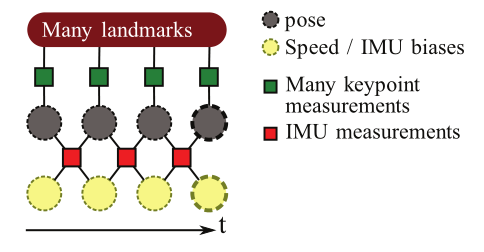
\includegraphics[width=.5\textwidth]{Pictures/okvis.png}
    \caption{OKVIS因子图示例图\citep{leutenegger2015keyframe}}
    \label{fig:okvis}
\end{figure}

和大部分的SLAM系统一样,IMU预积分技术的后端优化也是基于非线性最小二乘。它的能量函数同样包括基本的视觉观测项和IMU预积分项(见图~\ref{fig:preint}),形式上没有区别,区别仅在IMU部分的能量:
\begin{equation}\label{eq:gtsam_res}
    \bm{\mathcal X}^\star =
        \arg\mathop{\min}_{\bm{\mathcal X}}
        \sum_{i,j}\left\| \bm{r}_{\mathcal{I}_{ij}} \right\|^2_{\mathrm\Sigma_{ij}} +
        \sum_{i} \sum_{l} \left\| \bm{r}_{\mathcal{C}_{il}} \right\|^2_{\mathrm\Sigma_{C}}
\end{equation}

\begin{figure}[htb!]
    \centering
    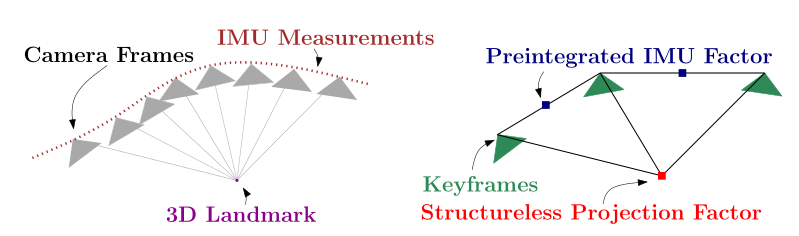
\includegraphics[width=.6\textwidth]{Pictures/preint.png}
    \caption{IMU预积分因子图示例\citep{forster2017manifold}}
    \label{fig:preint}
\end{figure}

其中$\bm{r}_{\mathcal{C}_{il}}$是关于状态$i$和路标点$l$的视觉部分目标函数,这一部分的定义和大部分SLAM系统一致。$\bm{r}_{\mathcal{I}_{ij}}$则与MSCKF、OKVIS等系统不同,是关于相邻状态$i$和$j$的IMU预积分目标函数。在IMU预积分技术中,这一项被认为是仅和状态$i$的偏移量相关的函数:$\Delta\tilde{\mathrm R}_{ij}(\bm{b}^g_i)$、$\Delta\tilde{\bm v}_{ij}(\bm{b}^g_i, \bm{b}^a_i)$和$\Delta\tilde{\bm p}_{ij}(\bm{b}^g_i, \bm{b}^a_i)$。前面已经给出了IMU预积分项的误差模型,因此可以很容易地写出IMU预积分项的目标函数:

\begin{equation}
\begin{aligned}
  \bm{r}_{\Delta\mathrm{R}}
    &\doteq
      \log\left(
        \left(
          \Delta\bar{\mathrm R}_{ij}
          \exp\left(
            \tfrac{\partial\Delta\bar{\mathrm R}_{ij}}{\partial\bm{b}^g_i}
            \delta\bm{b}^g_i\right)
        \right) \mathrm{R}^\top_i \mathrm{R}_j
      \right) \\
  \bm{r}_{\Delta\bm{v}}
    &\doteq
      \mathrm{R}^\top_i(\bm{v}_j - \bm{v}_i - \bm{g}\Delta t_{ij}) -
      \left[
        \Delta\bar{\bm v}_{ij} +
        \tfrac{\partial\Delta\bar{\bm v}_{ij}}{\partial\bm{b}^g_i}
        \delta\bm{b}^g_i +
        \tfrac{\partial\Delta\bar{\bm v}_{ij}}{\partial\bm{b}^a_i}
        \delta\bm{b}^a_i
      \right] \\
  \bm{r}_{\Delta\bm{p}}
    &\doteq
      \mathrm{R}^\top_i(
        \bm{p}_j - \bm{p}_i -
        \bm{v}_i \Delta t_{ij} -
        \tfrac{1}{2}\bm{g}\Delta t^2_{ij}) -
      \left[
        \Delta\bar{\bm p}_{ij} +
        \tfrac{\partial\Delta\bar{\bm p}_{ij}}{\partial\bm{b}^g_i}
        \delta\bm{b}^g_i +
        \tfrac{\partial\Delta\bar{\bm p}_{ij}}{\partial\bm{b}^a_i}
        \delta\bm{b}^a_i \right]
\end{aligned}
\end{equation}
 % section : 基于IMU预积分技术的VISLAM

\section{本章小结}

本章详细介绍了IMU传感器的基本模型,包括噪声模型和运动模型,并给出了基于IMU预积分方法的VISLAM基本原理。如前面提到的,由IMU预积分提供的观测可以和一般常用的VSLAM的视觉观测进行联合优化。本文提出的增量式舒尔补基数调整提供了基于IMU预积分的目标函数将连同重投影误差目标函数的实现。
